\chapter{Discussion}\label{ch:overall}\label{ch:futurework}
\graphicspath{{../Figures/70-overall/}{figs/70-overall/}}

\section{Overview}\label{sec:foundation}

Designing a robot knee for human-scale torque sets two different tests. With the joint fixed, the actuator and its route must transmit the required moment to the shank. During a step, the controller must recruit that actuator while the leg is in a position to accept or release load. A knee can meet the first requirement and still fail the second. The same distinction matters when using a robot to study biology. A change in foot loading after a sensory pathway is disabled has an interpretable cause only when the actuator, route, and external support are known.

I addressed these questions at four points in the design process. The actuator tests show how much tension a BPA of a given resting length can produce at a specified pressure and contraction. At the knee, that tension acts through a moment arm. The isometric tests showed how deflection under load changes the torque available from a proposed route. For controller design, I developed the Sensory Afferent Database (SADb) so a researcher can find the experiment behind a proposed feedback connection. The neuromechanical tools then let the researcher change that connection in a model and measure its effect on movement. Figure~\ref{fig:design_workflow} shows where each result enters a new design.

\begin{figure}[!htbp]
\centering
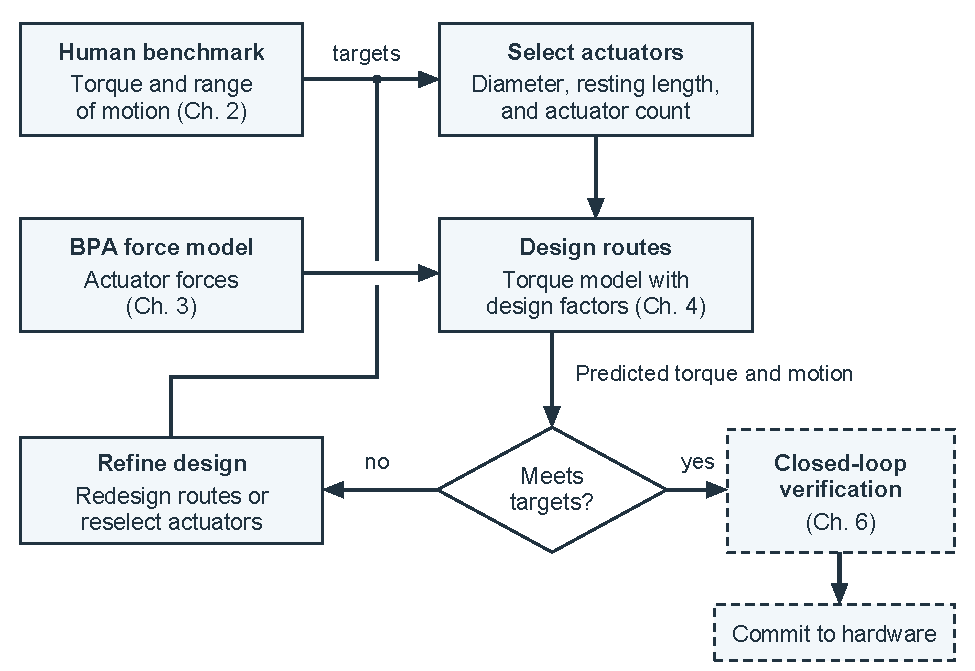
\includegraphics[width=\textwidth]{design_workflow.pdf}
\caption[Design workflow for a BPA-actuated joint]{Human torque and range-of-motion targets guide actuator sizing and route selection. Testing the resulting mechanical model with a controller precedes a commitment to hardware.}
\label{fig:design_workflow}
\end{figure}

\section{Research Contributions and Future Work}

\subsection{BPA Actuator Characterization}

Festo's sizing tool predicted that a shorter BPA would produce greater maximum force. On our isometric test jig, shorter actuators of the same diameter produced less maximum force at \qty{620}{\kPa} (Chapter~\ref{ch:muscles}, Figure~\ref{fig:Fmax_fit}). We used this measured dependence on resting length to scale a three-coefficient force surface fitted to normalized pressure and contraction. A designer can use the model to compare candidate actuator lengths at the pressure and contraction required by a joint, within the range we tested.

\subsubsection{Future Work}\label{sec:fw_bpa}

For a new actuator, free contraction at the reference pressure, $\varepsilon_{620}$, still has to be measured. The \qty{20}{\mm} specimens came from one batch. Testing several resting lengths within each batch and repeating the series across the \qtylist{10;20;40}{\mm} sizes would distinguish a length trend from manufacturing variation.

One explanation for the resting-length effect concerns the shape of the pressurized tube. Near each end fitting the outer diameter remains close to its uninflated value. It increases through a transition region to the nominal inflated diameter in the central span (Figure~\ref{fig:bpa_construction}A). If the transition occupies a similar axial length at a given pressure, a shorter actuator has a smaller fraction of its wall operating as a uniform cylinder. The physical end cap raises a different question. Measuring relative displacement across Onyx and aluminum caps under matched tensile loads, with the actuator pressurized and unpressurized, would isolate the contribution of cap and attachment compliance. An axial profile of tube diameter is needed to test the transition-region explanation.

Can deformation near the fittings account for the difference in isometric force between short and long actuators? I propose a geometrically nonlinear finite-element model for this question. Festo describes a pressure-sealing rubber wall reinforced by aramid fabric \citep[p.~2]{festo_2026}. I would represent the wall as a nearly incompressible hyperelastic material and the braid as two embedded families of tension-only truss elements following the measured fiber angles. A curved membrane can represent the taut central span when bending is negligible. A thin shell adds bending where curvature varies over distances large compared with wall thickness. A thick shell can represent transverse shear in a shorter transition, while mixed displacement--pressure solids through the thickness are appropriate where the fitting compresses the rubber or produces local contact stress. A flat plate would discard the circumferential load path. I would embed the fibers where they are bonded to the rubber and use measured frictional contact at a mechanically clamped interface that can slip. Sectioning a specimen and marking the wall relative to the fitting would distinguish bonded regions from sliding surfaces. Pressure would follow the deforming inner wall, with the closed-end pressure resultant included once, as the tube expands and the fiber angles change.

\begin{figure}[H]
\centering
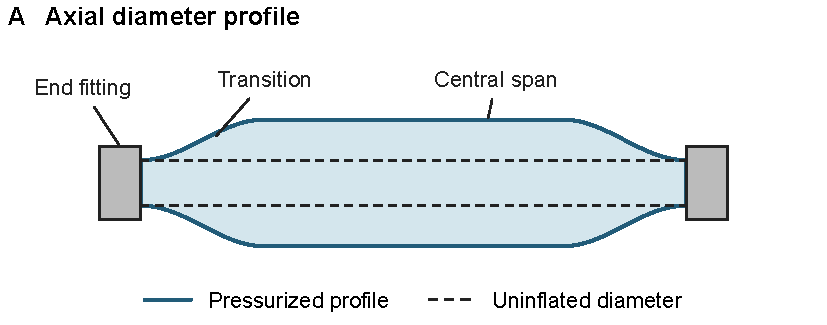
\includegraphics[width=14cm]{bpa_construction.pdf}\par\smallskip
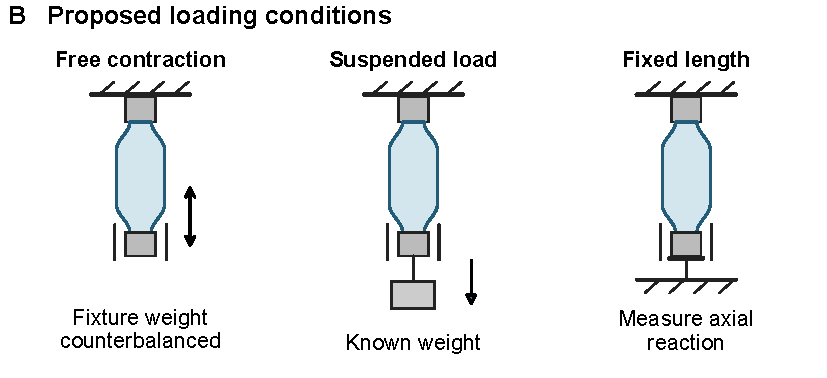
\includegraphics[width=14cm]{bpa_exploded_cutaway.pdf}
\caption[End deformation and proposed BPA experiments]{Proposed investigation of the end effect. (A) The fittings constrain the local diameter while the central span expands. The profiles show the geometric hypothesis. (B) An axial guide permits free or loaded shortening, while locking the guide gives an isometric force test. Diameter and fitting separation distinguish wall deformation from fitting motion.}
\label{fig:bpa_construction}
\end{figure}

I would prescribe the same measured gauge-pressure ramp from zero to \qty{500}{\kPa} for two quasi-static tests, fixing the upper fitting in both. For free contraction the lower fitting would translate along the axis with its fixture weight counterbalanced. For loaded contraction it would lift a known suspended mass with axial load $mg$, including the moving fixture in $m$. At each pressure plateau I would measure fitting separation, the diameter profile along the tube, and axial force at the fixed support. A third test would hold fitting separation fixed and measure the change in reaction with pressure. Agreement in the axial profile and the held-length force across resting lengths would test the end-effect hypothesis directly. Dynamic loading would then address a separate question about pressure response and hysteresis \citep{elzein_pressure_2025}. Appendix~\ref{app:muscle_calcs} gives the biological-muscle formulations used for comparison \citep{thelen_adjustment_2003,millard_flexing_2013}.

\subsection{Isometric Joint Design Factors}

On the biomimetic knee, the original rigid-body model overpredicted the torque from the extensor route (Chapter~\ref{ch:torque}). I accounted for length offsets, compliance in the loaded force path, and the loss of usable BPA length where it wraps. The fitted stiffness pair includes the compliance of the fixtures and the loading connection. I then used the corrected model to size two routes and tested them on the knee. At the sampled angles, the flexor met or exceeded the isometric torque magnitude of the Gait2392 biceps femoris short head, and the extensor met or exceeded that of the vastus medialis. These tests extend earlier work on geometric attachment placement \citep{bolen_bipedal_2019,bolen_determination_2019,morrow_optimization_2020} by checking the torque each route delivers under load.

\subsubsection{Future Work}\label{sec:fw_routing}

In a pulley-assisted BPA route, a fixed pulley redirects tendon tension. A multi-part tackle also changes the relation between actuator travel and insertion force and needs space for the moving pulleys (Appendix~\ref{sec:app_routing_extensions}). A cam or artificial patella can change the moment arm as the knee flexes. To test that design, I would measure knee-axis torque and tendon tension on both sides of the contact across a knee-angle sweep. Recording the angles at which the tendon engages and leaves the cam would show where any discrepancy from the predicted torque occurs.

Isometric tests establish torque capacity at zero angular velocity. To determine when that capacity can do work, I would measure knee torque $\tau$ and angular velocity $\omega$ on the same time base and about the same signed axis. Their product $P=\tau\omega$, in watts, is the instantaneous mechanical power delivered by the knee to the external load. Positive power indicates energy delivery and negative power indicates absorption. Its timing and magnitude distinguish a knee that supplies energy during extension from one that resists motion to absorb a landing load. A biomechanist can compare these phases with joint-power profiles, and a robot designer can size the actuator for both propulsion and controlled deceleration. A dynamometer on the test stand could drive flexion and extension at prescribed speeds or impose a resisting torque while the BPA moves the knee. An encoder and a joint-axis torque transducer would supply synchronized velocity and torque. Recording actuator pressure and calibrating fixture inertia, friction, and loading-connection compliance would help distinguish pneumatic delay and load--unload hysteresis from losses in the rig.

\subsection{Sensory Afferent Database}

In the SADb a researcher can trace a proposed connection to the stimulus and response that support it, then compare the preparations in which the response changed. In the Table view, selecting \emph{Ib disynaptic excitation} under \emph{Pathway} returns linked papers. The record for \citet{mccrea_disynaptic_1995} opens a curation note, its pathway links, and the article DOI. In decerebrate cats, stimulating the plantaris nerve inhibited medial gastrocnemius motoneurons at rest. During the extensor phase of midbrain-evoked fictive locomotion, the same stimulation excited these synergist motoneurons. In an acute spinal preparation treated with clonidine, inhibition decreased without the short-latency excitation. The record also links to \emph{Ib disynaptic inhibition}. Reading the original experiment shows why those two links belong together and why a controller designer would test a state-dependent group~I pathway. The stimulation recruited group~I afferents and did not isolate Ib input.

\subsubsection{Future Work}\label{sec:fw_database}

The monthly literature watch supplies candidates for manual curation (Section~\ref{sec:sadb_methods}). For a pathway such as extensor group~I excitation, the most useful addition to a record would be a direct link from each reported sign to its preparation, stimulus, and phase. A reader could then distinguish a measured reversal from an assumption in a computational model before following their citation links. The Bubble map already identifies citation communities by color. Grouping their papers spatially would provide a second way to locate related studies \citep{bolen_using_2024}.

\subsection{SNS Tools and Neuromechanical Experiments}

Morrow and I first transferred the Deng controller to the Li walker in AnimatLab. The legs cycled while suspended and the model tipped when released. The result motivated a practical change in how I tested controllers. I built tools to follow one signal from sensory input through the neural circuit to actuator force and joint motion. In the knee example an extensor Ia pulse produces a measurable extension and recovery. In the supported W2L model, removing the specified sensory inputs and conductances displaced footfalls from antiphase while the body continued to move forward. Recording both contact and movement made the coordination deficit observable.

The human-model drive experiment tested a different dependence. The human model continued to step in place under its support rig with the supplementary left and right hand-drive channels set to zero and the shared descending drive still active. A separate W2L robot model progressed with reduced supplementary drive under its harness (Section~\ref{sec:sns_controller_comparison}). These tests identify which command was removed and what mechanical support the remaining controller had to work against.

\subsubsection{Future Work}\label{sec:fw_pipeline}\label{sec:fw_cpg}

A next controller-transfer test would stimulate the same RG, PF, or MN pathway under prescribed sensory replay and during closed-loop motion. A phase shift at the rhythm generator would distinguish a reset from a skipped motor burst with preserved rhythm (Section~\ref{sec:app_layer_stimulus}). Physiological and modeling studies provide reference responses for such experiments \citep{selionov_tonic_2009,rybak_modelling_2006,markin_afferent_2010,shevtsova_modeling_2016}. Repeating the protocol with the same unaffected synaptic gains, mechanical support, and perturbation would locate where the responses diverge.

\paragraph{Sensory and Higher-Level Control}\label{sec:fw_senses}

In earlier BPA balance-platform experiments, orientation feedback provided a hardware precedent for estimating body attitude \citep{hilts_dynamic_2019,bolen_balance_2024,bolen_selfbalancing_2024,bolen_selfbalancing_srs_2024}. For the biped I would first test whether an estimate of trunk orientation and angular velocity improves recovery from a repeatable disturbance at fixed harness assistance. Adding a visual reference in a second condition would test the effect of correcting inertial drift under the same disturbance. The expected contribution of each signal depends on the task \citep{akay_relative_2021}. Figure~\ref{fig:sensorium_hierarchy} places these proposed pathways above the implemented spinal network.

Once spinal timing is repeatable, adaptive step length provides an observable task for a higher-level controller. Multilevel controllers for insect-like legs \citep{grummer_multilevel_2024} and a cortico-cerebellar-spinal model of step-length adaptation \citep{chen_corticocerebellar_2025} suggest mechanisms for coordinating or adapting successive steps. A useful first comparison would measure the size and persistence of the correction to a repeated perturbation with and without the proposed adaptive pathway.

\begin{figure}[H]
\centering
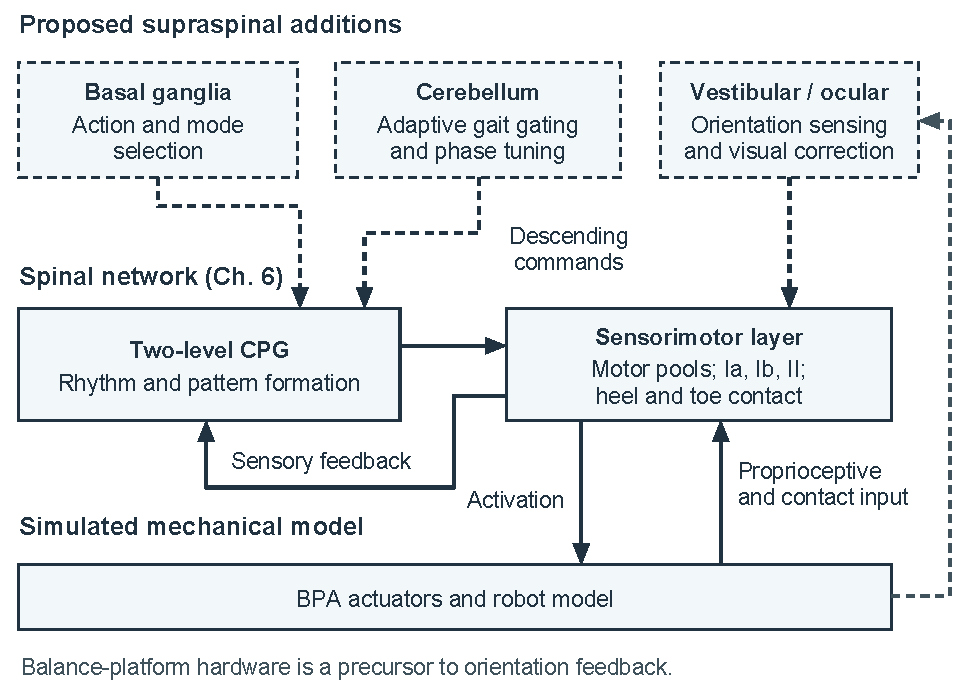
\includegraphics[width=0.96\textwidth]{sensorium_hierarchy.pdf}
\caption[Control stack with the planned supraspinal additions]{Control hierarchy connecting spinal pathways and the BPA-actuated model to proposed supraspinal and sensory extensions. Dashed elements indicate future work.}
\label{fig:sensorium_hierarchy}
\end{figure}

\paragraph{Hardware Transfer}\label{sec:fw_hardware}

Figure~\ref{fig:pipeline} shows the next interface to test before connecting the physical biped. In a controller hardware-in-the-loop test, a real-time simulation of the leg would send sensory measurements to the embedded controller and receive its actuator commands. Replaying the same perturbation through the software and embedded controllers would expose sample delays, missed updates, or scaling errors. Figure~\ref{fig:simulation_workflow} identifies the simulation interfaces already available for that comparison.

\begin{figure}[H]
\centering
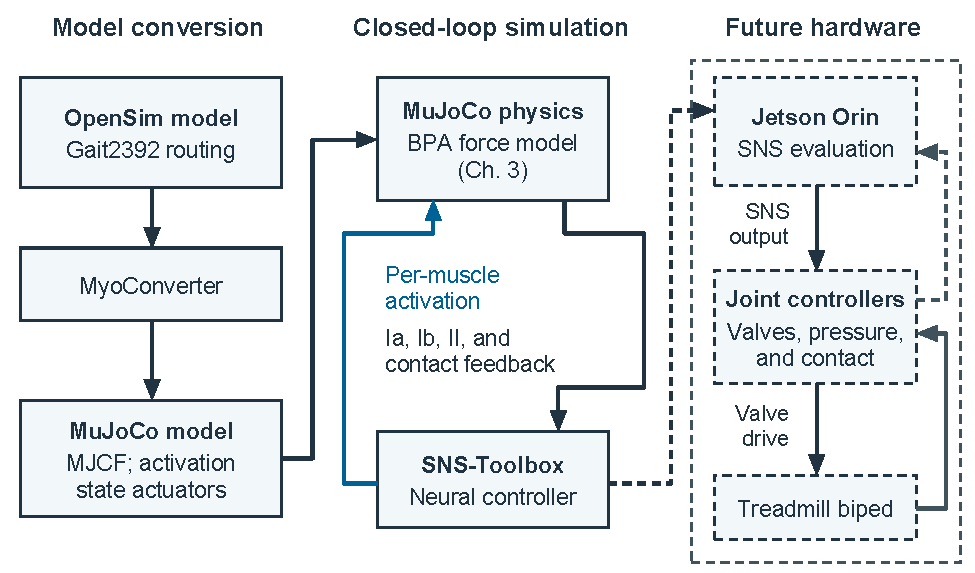
\includegraphics[width=\textwidth]{pipeline.pdf}
\caption[Simulation-to-hardware workflow]{Model conversion, closed-loop simulation, and proposed hardware deployment. Simulation interfaces exchange actuator commands and afferent signals. The embedded valve-control and network-evaluation system and treadmill deployment are future work.}
\label{fig:pipeline}
\end{figure}

In the proposed hardware implementation, Teensy-class microcontrollers would handle joint-level measurements and valve commands, and an NVIDIA Jetson Orin would evaluate the neural circuit. I would reconstruct length and velocity from encoders and the calibrated path geometry, and use measured tension for force feedback. Pressure transducers, foot contacts, and inertial measurements would complete the channels required by the selected controller. Recording time from each sensor sample to the resulting pressure response would test whether measured delays preserve the corrective response observed in simulation \citep{elzein_pressure_2025}.

Physical PAM-biped control \citep{li_controller_2024} and transfer of Muscle Mutt's SNS controller from MuJoCo to hardware \citep{lutz_mechanical_2025} provide precedents for this experiment. The comparison for this biped would be the measured joint and contact response to the same input, with its own actuator routes and sensors.

\paragraph{Dynamic Whole-Body Maneuvers}\label{sec:fw_kickflip}

My longer-term goal is a robot that can perform a kickflip. The knee must deliver power during takeoff, the controller must estimate orientation in the air, and the legs must absorb energy when contact resumes. Those are three identifiable experiments on the way from a stationary torque measurement to a coordinated whole-body maneuver.

\section{From Design Tools to Neuromechanical Experiments}

The four contributions make it possible to ask where a proposed controller and a particular leg first disagree. A force shortfall at a known pressure points to actuator or route mechanics. Correct force with a mistimed footfall points to recruitment, sensory encoding, or the support condition. The measurements and interventions developed here allow those explanations to be tested separately.
